Consider the case of Consonantal Nasal harmony in Yaka  \cite{Walker_Yaka}: \\- a nasal stop induces nasalization of voiced consonants (Cs) occurring at any distance to its right.
As can be seen from the  segmental alternation in  Ex.~(\ref{ex:1}),  the phoneme \textipa{/d/} surfaces as  \textipa{[n]} after a nasal  (cf.  Ex.~(\ref{ex:1a}, \ref{ex:1b} vs.  \ref{ex:1c})).
Vowels and voiceless consonants intervening between the two harmonizing stops remain unaffected  (cf. Ex.~(\ref{ex:2})).


\begin{exe}
    \ex\label{ex:1}\begin{xlist}
    	 \ex\label{ex:1a} \textipa{yan-ini}   
	 \ex\label{ex:1b} \textipa{yad-idi}
	 \ex\label{ex:1c} $^*$\textipa{yan-idi}      
	\end{xlist}
    \ex\label{ex:2}\begin{xlist}
     	\ex\label{ex:2a}\textipa{hamuk-ini} 
    	\ex\label{ex:2b}\textip{miituk-ini}
    \end{xlist}
     \ex\label{ex:3}\begin{xlist}
    	 \ex\label{ex:3a}    \textipa{biimb-idi}
	 \ex\label{ex:3b}  \textipa{kuund-idi}
	 \ex\label{ex:3c}  \textipa{naang-ini}
	\end{xlist}
\end{exe}

A TSL analysis for this patter seems straightforward, as this data can be captured by projecting a tier of voiced consonants, and enforcing constraints banning tier adjacent  \textipa{[nd]}.

\begin{figure}[t]
\centering
    \begin{tikzpicture}

\node (A) at (-1,1.4) {\textbf{(a)}};
\node (00) at (-0.4,0.1) {$^{*}$};
\node (0) at (0,0) {s};
\node (1) at (0.5,0) {n};
\node (2) at (1,0) {i};
\node (3) at (1.5,0) {\textglotstop};
%%tier
\node (00) at (0,1) {s};
\node (01) at (0.5,1) {n};
\node (000) at (-0.5,1.3) {$^*$};
\draw [dashed, red] (-0.3, 0.7) -- (0.7, 0.7) -- (0.7,1.3) -- (-0.3,1.3) -- (-0.3, 0.7);
\draw[dotted, thick, blue] (-0.35,0.60) to (1.8,0.60);
%\node at (-0.3,0.40) {{\tiny T}};
%
\end{tikzpicture}
   %    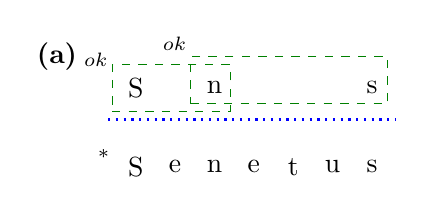
\begin{tikzpicture}
\node (A) at (-1.5,1.4) {\textbf{(a)}};
\node (00) at (-0.9,0.1) {$^{*}$};
\node (0) at (-0.5,0) {\textipa{S}};
\node (0) at (0,0) {e};
\node (1) at (0.5,0) {n};
\node (2) at (1,0) {e};
\node (3) at (1.5,0) {t};
\node (4) at (2,0) {u };
\node (5) at (2.5,0) {s};
%
\node (00) at (-0.5,1) {\textipa{S}};
\node (01) at (0.5,1) {n};
\node (03) at (1.5,1) {};
\node (5) at (2.5,1) {s};
%
\node (000) at (-1,1.3) {$^{ok}$};
\draw [dashed, green!50!black] (-0.8, 0.7) -- (0.7, 0.7) -- (0.7,1.3) -- (-0.8,1.3) -- (-0.8, 0.7);
\node (000) at (0,1.5) {$^{ok}$};
\draw [dashed, green!50!black] (0.2, 0.8) -- (2.7, 0.8) -- (2.7,1.4) -- (0.2,1.4) -- (0.2, 0.8);

\draw[dotted, thick, blue] (-0.85,0.60) to (2.8,0.60);
%   \node at (-0.3,0.40) {{\tiny T}};
    
\end{tikzpicture}
 
        %
       \hspace{2cm}
    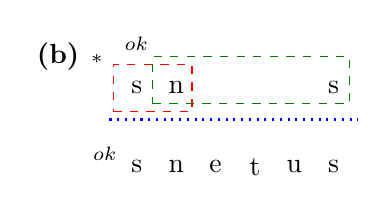
\begin{tikzpicture}
\node (A) at (-1,1.4) {\textbf{(b)}};
\node (00) at (-0.4,0.1) {$^{ok}$};
\node (0) at (0,0) {s};
\node (1) at (0.5,0) {n};
\node (2) at (1,0) {e};
\node (3) at (1.5,0) {t};
\node (4) at (2,0) {u };
\node (5) at (2.5,0) {s};
%
\node (00) at (0,1) {s};
\node (01) at (0.5,1) {n};
\node (03) at (1.5,1) {};
\node (5) at (2.5,1) {s};
%
\node (000) at (-0.5,1.3) {$^{*}$};
\draw [dashed, red] (-0.3, 0.7) -- (0.7, 0.7) -- (0.7,1.3) -- (-0.3,1.3) -- (-0.3, 0.7);
\node (000) at (0,1.5) {$^{ok}$};
\draw [dashed, green!50!black] (0.2, 0.8) -- (2.7, 0.8) -- (2.7,1.4) -- (0.2,1.4) -- (0.2, 0.8);

\draw[dotted, thick, blue] (-0.35,0.60) to (2.8,0.60);
%   \node at (-0.3,0.40) {{\tiny T}};
    
\end{tikzpicture}
    
        \caption{Example of a TSL analysis of nasal harmony in Samala: (a) is ill-formed because of adjacent $^*$\textipa{[nd]}; (b) is well-formed since  \textipa{[n]} is followed by another  \textipa{[n]} later in the string; (c) is well-formed because the \textipa{[nd]} cluster does not enforce nasality on the following stops, but it is still ruled out by the constraint needed for (b). }
        \label{fig:YAKA1}
        \end{figure}



However, observe now the examples in  Ex.~(\ref{ex:3}): consonantal complexes composed of a nasal and a voiced oral stop neither trigger   Ex.~(\ref{ex:3a},\ref{ex:3b}) nor block nasality agreement   Ex.~(\ref{ex:3c}).
Fig.~\ref{fig:YAKA1} exemplifies why this interaction of a local and a non-local dependency is not TSL\@. 
Since \textipa{[nd]} is sometimes observed in a string-adjacent context (as in Ex.~(\ref{ex:3b})), it must be permitted as a $2$-gram on a tier --- even though it is only allowed when  \textipa{[nd]} re immediately adjacent in the string.
But then,  a TSL grammar would have no means of distinguishing Ex.~(\ref{ex:1b}) from Ex.~(\ref{ex:3b}).

The reader might point out that the difference between Fig.~ \ref{fig:YAKA1}.a and Fig.~ \ref{fig:YAKA1}.c can be resolved by extending the tier-grammar to consider $3$-grams.
However, in order to enforce harmony correctly, the tier-projection places every occurrence of voiced stops in the string on the tier, thus making $3$-grams constraints insufficient (e.g., Ex.~(\ref{ex:3}c)).
Thus, since the number of segments between harmonizing elements is potentially unbounded, no TSL grammar can generally account for this pattern, independently of the dimension of the tier $k$-grams.

Consider now the examples in Ex.~(\ref{ex:3}). 
We know that the nasals immediately followed by a viced stop do nt trigegr harmony, and that said stop does not harmonize. 
Moreover, since they do not block the harmonic process, these consonants do no participate in the harmony at all.
Thus, if we could make projection of nasal and stops to avoid  those segments that appear in specific consonant clusters (e.g. \textipa{[nd]}) the tier constraints discussed above would work once again.
This is not possible with TSL as originally defined in \cite{HeinzRawalTanner}, as TSL selects tier elements only based on their $1$-local properties (i.e. which kind of segment they are). %Sec.~\ref{sec:SSTSL}.
The intuition is that we can make a TSL grammar  simultaneously aware of local and non-local properties of segments in the string with a natural change to the definition of the erasing function.
This kind of expressivity can be accomplished by increasing the locality window of the \emph{tier projection mechanism}. 

\begin{figure}[]
\begin{center}
    %\begin{tikzpicture} %SSTSL EXAMPLE
    \node (A) at (-1.2,1.4) {\textbf{(b)}};
      \node (60) at (-0.5,0) {$\rtimes$};
        \node (0) at (0,0) {s};
        \node (1) at (0.5,0) {n};
        \node (2) at (1,0) {e};
        \node (3) at (1.5,0) {t};
        \node (4) at (2,0) {u };
        \node (5) at (2.5,0) {s};
      \node (6) at (3,0) {$\ltimes$};
        %%tier
             \node (600) at (-0.5,1) {$\rtimes$};
       \node (00) at (0,1) {s};
       \node (01) at (0.5,1) {n};
       \node (5) at (2.5,1) {s};
          \node (06) at (3,1) {$\ltimes$};
        %
        %projection function
       \draw[dashed, blue] (-0.7,-0.28 ) rectangle (0.25, 0.28);
         \draw  [dashed, blue] (-0.2,-0.2 ) rectangle (0.65, 0.2);
         \draw [dashed, blue](2.25,-0.28 ) rectangle (3.25, 0.28);
          %local constraints   
 	 \node (000) at (-0.6,1.3){$^{ok}$};
        \draw [dashed, green!50!black](-0.3, 0.7) -- (2.7, 0.7) -- (2.7,1.3) -- (-0.3,1.3) -- (-0.3, 0.7);
        %tier bar
        \draw[dotted, thick, blue] (-0.65,0.60) to (3.3,0.60);
       % \node at (-0.5,0.40) {{\tiny T}};
        
        \begin{scope}[xshift=-180pt] %string in the center
         \node (A) at (-1.2,1.4) {\textbf{(a)}};
         \node (60) at (-0.5,0) {$\rtimes$};
        \node (0) at (0,0) {s};
        \node (1) at (0.5,0) {n};
        \node (2) at (1,0) {i};
        \node (3) at (1.5,0) {\textglotstop};
         \node (6) at (2,0) {$\ltimes$};
        %%tier
          \node (600) at (-0.5,1) {$\rtimes$};
        \node (00) at (0,1) {s};
        \node (01) at (0.5,1) {n};
          \node (006) at (2,1) {$\ltimes$};
        %projection function
        \draw[dashed, blue] (-0.7,-0.28 ) rectangle (0.25, 0.28);
        \draw  [dashed, blue] (-0.2,-0.2 ) rectangle (0.65, 0.2);
	%local constraints
        \node (000) at (-0.5,1.3) {$^*$};
        \draw [dashed, red] (-0.3, 0.7) -- (2.25, 0.7) -- (2.25,1.3) -- (-0.3,1.3) -- (-0.3, 0.7);
      \draw[dotted, thick, blue] (-0.65,0.60) to (2.5,0.60);
       % \node at (-0.5,0.40) {{\tiny T}};
        %
        \end{scope}
        
        \end{tikzpicture}

    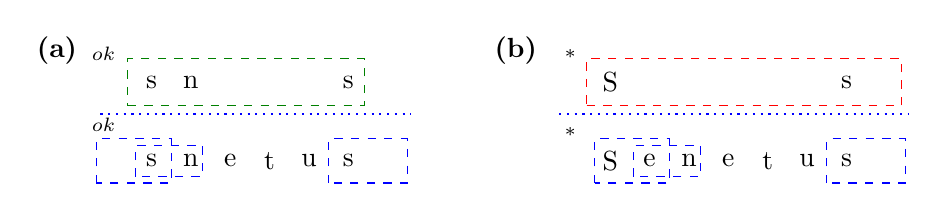
\begin{tikzpicture} %SSTSL EXAMPLE
    \node (A) at (-1.7,1.4) {\textbf{(b)}};
    \node (6000) at (-1,0) {$\rtimes$};
      \node (60) at (-0.5,0) {\textipa{S}};
        \node (0) at (0,0) {e};
        \node (1) at (0.5,0) {n};
        \node (2) at (1,0) {e};
        \node (3) at (1.5,0) {t};
        \node (4) at (2,0) {u };
        \node (5) at (2.5,0) {s};
      \node (6) at (3,0) {$\ltimes$};
        %%tier
         \node (6000) at (-1,1) {$\rtimes$};
             \node (600) at (-0.5,1) {\textipa{S}};
     %  \node (00) at (0,1) {s};
    %   \node (01) at (0.5,1) {n};
       \node (5) at (2.5,1) {s};
          \node (06) at (3,1) {$\ltimes$};
        %
        %projection function
       \draw[dashed, blue] (-0.7,-0.28 ) rectangle (0.25, 0.28);
         \draw  [dashed, blue] (-0.2,-0.2 ) rectangle (0.65, 0.2);
         \draw [dashed, blue](2.25,-0.28 ) rectangle (3.25, 0.28);
          %local constraints   
 	  \node (000) at (-1,1.3) {$^*$};
	    \node (0000) at (-1,0.3) {$^*$};
        \draw [dashed, red](-0.8, 0.7) -- (3.2, 0.7) -- (3.2,1.3) -- (-0.8,1.3) -- (-0.8, 0.7);
        %tier bar
        \draw[dotted, thick, blue] (-1.15,0.60) to (3.3,0.60);
       % \node at (-0.5,0.40) {{\tiny T}};
        
        \begin{scope}[xshift=-180pt] %string in the center
         \node (A) at (-1.2,1.4) {\textbf{(a)}};
        \node (0) at (0,0) {s};
        \node (1) at (0.5,0) {n};
        \node (2) at (1,0) {e};
        \node (3) at (1.5,0) {t};
        \node (4) at (2,0) {u };
        \node (5) at (2.5,0) {s};
      \node (6) at (3,0) {$\ltimes$};
        %%tier
             \node (00) at (-0.5,0) {$\rtimes$};
             \node (600) at (-0.5,1) {$\rtimes$};
       \node (00) at (0,1) {s};
       \node (01) at (0.5,1) {n};
       \node (5) at (2.5,1) {s};
          \node (06) at (3,1) {$\ltimes$};
        %
        %projection function
       \draw[dashed, blue] (-0.7,-0.28 ) rectangle (0.25, 0.28);
         \draw  [dashed, blue] (-0.2,-0.2 ) rectangle (0.65, 0.2);
         \draw [dashed, blue](2.25,-0.28 ) rectangle (3.25, 0.28);
          %local constraints   
 	 \node (000) at (-0.6,1.3){$^{ok}$};
	  \node (0000) at (-0.6,0.4){$^{ok}$};
        \draw [dashed, green!50!black](-0.3, 0.7) -- (2.7, 0.7) -- (2.7,1.3) -- (-0.3,1.3) -- (-0.3, 0.7);
        %tier bar
        \draw[dotted, thick, blue] (-0.65,0.60) to (3.3,0.60);        %
        \end{scope}
        
        \end{tikzpicture}

        \end{center}
        % \caption{Example from Samala, allowing generalized tier projection: (a) is ill-formed because of $^*$\textipa{sn}; (b) is well-formed since  \textipa{[sn]} is followed by \textipa{[s]} later in the string. Note that \textipa{[n]} is projected on the tier only when adjacent to \textipa{[s]}.}
         %if changed to new fig
        \caption{Example of a TSL analysis of nasal harmony in Samala: (a) is ill-formed because of adjacent $^*$\textipa{[nd]}; (b) is well-formed since  \textipa{[n]} is followed by another  \textipa{[n]} later in the string; (c) is well-formed because the \textipa{[nd]} cluster does not enforce nasality on the following stops.  Note that \textipa{[n,d]} are projected on the tier only when not immediately adjacent in the input. }
        \label{fig:YAKA2}
        \end{figure}


Fig.~\ref{fig:YAKA2} shows how, by increasing the locality of the projection to $2$, we allow the grammar to project a nasal iff it is not immediately followed by a voiced oral stop, and then use $2$-local tier constraints to ban  \textipa{nd}.%
This time,  possible intermediate clusters are not a problem, since the projection is able to infer that they are in local contexts that make them irrelevant to the harmonic process.

Finally, note the following additional data:


\begin{exe}
    \ex\label{ex:4}\begin{xlist}
    	 \ex\label{ex:4a} \textipa{kem-ene}   
	 \ex\label{ex:4b} \textipa{keb-ede}
	\end{xlist}
\end{exe}

Ex.~(\ref{ex:4}) shows a vowel alternation that is independent of the nasality process, and is instead due to vowel heigh harmony.
Vowel harmony can be easily accounted for with a TSL grammar.
However, this is only true if we analyze it by itself, and fails if we try to model nasal harmony and vowel harmony in a single grammar.
In order to account for this, vowel will need to be projected on the tier, thus interfering with the nasalization process.
This issue is resolved working with the intersection closure of ITSL languages (MITSL).

Since the ability to model multiple processes in the phonotactic of a language remains obviously desirable, it seems reasonable then to focus on the learnability of MITSL languages directly, as any algorithm able to learn an MITSL language will also trivially learn an ITSL one.